\documentclass[14pt]{article}

\usepackage[utf8x]{inputenc}
\usepackage[russian]{babel}
\usepackage{graphicx}
\graphicspath{{images/}}
\DeclareGraphicsExtensions{.pdf,.png,.jpg}

\usepackage{amsmath}
\usepackage{pgfplots}

\usepackage{geometry} % Меняем поля страницы
\geometry{left=2cm}% левое поле
\geometry{right=1.5cm}% правое поле
\geometry{top=2cm}% верхнее поле
\geometry{bottom=2cm}% нижнее поле

\renewcommand{\theenumi}{\arabic{enumi}}% Меняем везде перечисления на цифра.цифра
\renewcommand{\labelenumi}{\arabic{enumi}}% Меняем везде перечисления на цифра.цифра
\renewcommand{\theenumii}{.\arabic{enumii}}% Меняем везде перечисления на цифра.цифра
\renewcommand{\labelenumii}{\arabic{enumi}.\arabic{enumii}.}% Меняем везде перечисления на цифра.цифра
\renewcommand{\theenumiii}{.\arabic{enumiii}}% Меняем везде перечисления на цифра.цифра
\renewcommand{\labelenumiii}{\arabic{enumi}.\arabic{enumii}.\arabic{enumiii}.}% Меняем везде перечисления на цифра.цифра

\begin{document}
\begin{titlepage}
	\begin{center}
		\fontsize{18pt}{20pt}\selectfont
		\textbf{Работа 1.1.4.}	
	
		\vspace{5cm}
		\fontsize{24pt}{25pt}\selectfont
		Измерение интенсивности радиационного фона
	\end{center}
	\begin{flushright}
		\fontsize{18pt}{20pt}\selectfont
		\vspace{14cm}
		\hspace{-3cm}
		\textit{Корнеев Е.С.}
	\end{flushright}		
\end{titlepage}

\begin{center}
	\fontsize{16pt}{18pt}\selectfont	
	Измерение интенсивности радиационного фона
\end{center}

\fontsize{14pt}{16pt}\selectfont
\vspace{1cm}
\textbf{Цель работы:} применение методов обработки эспериментальных данных для изучения статистических закономерностей при измерении интенсивности радиационного фона.

\vspace{0.5cm}
\textbf{В работе используются:} счетчик Гейгера-Мюллера, блок питания, компьютер с интерфейсом связи со счетчиком.

\vspace{1cm}
Случайный разброс результатов измерений может быть связан как с погреностью измерений, так и со случайными изменениями самой измеряемой величины. Поток космических частиц, которые составляют большую часть радиационного фона, изменяется со временем случайным образом. Если изменения происходят около какого-то значения, то говорят, что величина флуктуирует. В таком случае характеристиками этой величины в целом являются ее среднее значение и среднеквадратичное отклонение от того среднего. Для нахождения среднего значения и среднеквадратичного отклонения применяются те же методы, которые используются при рассчете средних значений и случайных погрешностей измерений.

\vspace{0.5cm}
Космические лучи разделяют на первичные, которые приходят на орбиту Земли из космоса, и вторичные, которые возникают лагодаря взаимодействию первичных с атмосферой Земли и составяляют основную часть космических лучей, доходящих до поверхности Земли. 

Подавляющая часть первичны лучей приходит к Земле из Галактики и лишь небольшая часть связана с активностью Солнца. О механизме возникновения космических лучей в Галактике пока существуют лишь гипотезы. Часть излучения возникает в звездах Галактики также, как на Солнце во время хромосферных вспышек. Более мощное излучение, по-видимомму, связано со вспышками сверхновых звезд и образующимися при это мпульсарами. Большую роль в ускорении космических частиц могут играть возникающие при вспышках свехновых звезд плазменные облака, двигающиейся с огромными скоростями, и галактические магнитные поля.

Первичные космические лучи --- потом стабильных частиц, имеющих большую юкинетическую энергию, которая составляет от $10^9$ до $10^{21}$ эВ. Установлено, что во всем пространстве поток частиц одинаков по всем направлениям (изотропен).

\vspace{0.5cm}
Основной величиной, характерихующих количество частиц в космических лучах, является интенсивность $I$. По определению интесивность есть часли частиц, падающих в единицу времени на единичную площадку, перпендикулярную к направлению наблюдения, отнесенное к единице телесного угла (стерадиану). Единицей измерения при этом является

$$\frac{\text{число частиц}}{\text{см}^2 \cdot cp \cdot c}$$

В случае изотропного распределения направлений космических лучей, что действительно имеет место вне атмосферы Земли, плотность $F$ потока частиц (из полусферы направлений) равна

$$F = 2\pi \int_0^{2\pi} I \cos(\theta)\sin(\theta)d\theta = \pi I~\left(\frac{\text{число частиц}}{\text{см}^2 \cdot cp \cdot c}\right)$$

\noindent Концентрация частиц, имеющих абсолютное значение скорости $V$:

$$n = \frac{4\pi I}{V} \left(\frac{\text{число частиц}}{\text{см}^3}\right)$$

\noindent Отметим, что подавляющее большинство частиц вне атмосферы движется со скоростями, близкими к скорости света, поэтому для оценки концентрации $n$ вместо $V$ можно использовать скорость света $c$. Отметим также, что вблизи поверхности Земли интенсивность космического излучения пропорциональна $cos^2(\theta)$, где $\theta$ --- угол с вертикалью. 

Плотность потока частиц измеряется колическом частиц, проходящих за 1 секунду через площадку в 1 $\text{см}^2$. На расстоянии порядка 50 км над поверхностью Земли плотность потока частиц равна приблизительно $1 \text{частица}/\text{см}^2 \cdot c$. Большую часть потока здесь составляют частицы с энергией порядка 10 ГэВ, частицы с меньшей энергией практически отсутствуют, что, видимо, связано с влиянием магнитных полей Земли и Солнечной системы. 

\vspace{0.5cm}
В основном первичные космические лучи состоят их протонов (92\%) и ядер гелия (6.6\%)б называемых $\alpha$-частицами. Обнаружены и более тяжелые ядра (вплоть до никеля), составялющие в сумме около 0.8\%.	Электронов и позитронов набирается примерно 1\%, причем позитронов в 10 раз меньше, чем электронов. Число $\gamma$-квантов с энергиями больше $10^8$ эВ составляет всего 0.01\%.

\vspace{0.5cm}
Временные изменения интенсивности потока первичных космических лучей невелики. Их изменения в основном для частиц порядка 1 ГэВ связаны с изменениями магнитных полей в Солнечной системе, вызываемых 11-летними циклами солнечной активности, 27-дневным периодов вращения Солнца вокруг своей оси, а также хромосферными вспышками на Солнце (5-13 вспышек в активный год) и магнитными бурями в магнитосфере Земли. Попадая в атмосферу Земли, первичные космические лучи взаимодействуют с ядрами атомов атфосферных газов и образуют вторичные космические лучи. Из 100 000 протонов первичных космических лучей до поверхности Земли доходит только один. Но появляются вторичные протоны, которые весте с мюонами и нейтронами составляют так называемую жестку компоненту космически лучей. Жестким называется излучение, прохоящее через свинцовую пласину толщиной 10 см. 

Мягкая компонента (задерживаемая свинцовой пластиной), состоит в основном из электронов, позитронов и фотонов. Мягкая комнонента существует вблизи поверхности Земли лишь потому, что она генерируется жесткой. Плотность потока мйгкой компоненты космических лучей с увеличением высоты возрастает быстрее, чем жесткой. На уровне моря плотность потока мягкой компоненты в вертикальном направлении составляет примерно половину плотности потока жесткой компоненты, которая равна $1.7 \cdot 10^{-2} \text{частиц}/\text{см}^2 \cdot c$, а на высоте 15 км плотность мягкой компоненты в 4-5 раз больше, чем жесткой. Общая плотность потоков максимальна на выоте приблизительно 17 км. В целом космические лучи на уровне моря приблизительно в 100 раз менее плотны, чем на верхней границе атмосферы, и на 2/3 состоят из мюонов. Анализ дна океана показал, что в среднем плотность потока не изменилась за последние 35 тысяч лет. 

Плотность потока лучшей вблизи поверхности земли сильно зависит от направления. Она максимальна в вертикальном и минимальна в горизонтальном, что связано с увеличением пути, проходимого лучами в атмосфере. Небольшие изменения плотности потока вторичных космических лучей со временм вызваны изменениями в атмосфере Земли давления, температуры и магнитных полей. 

\vspace{0.5cm}
В настоящее время, хотя уже построены мощные ускорители частиц, космические лучи остаются единственным источником частиц сверхвысоких энергий. Но приходят такие частицы не часто. Частица с энергией $10^{19}$ эВ пролетает через площадь в один квадратный метр вблизи земной поверхности один раз в 2 тысячи лет. Конечно, если площадь увеличить, например, до 10 квадратных километров, то это будет происходить один раз в несколько дней. Частицы больших энергий можно зарегистрировать по издаваемому ими вторичному потоку частиц, называемому атмосферными ливнями часпщ. Общее число частиц в ливне, зарождаюшемся на высоте примерно в 20—25 км над Землей, может достигать многих миллионов и покрывтъ площадь в несколько квадратных километров. Одновременное появление большого числа частиц на значительной площади служит подтверждением их общего происхождения и позволяет установить энергию образовавшей их частицы.

Космические лучи и естественная радиоактивность Земли и воздуха являются основным источником ионов в нижней части атмосферы Земли (до высот порядка 60 км). Ионизация в атмосфере с увеличением высоты вначале падает, а выше 1 км начинает возрастать, особенно резко с высоты 3 км. На высоте 5 км число ионов в единице объема в 3—4 раза больше, чем вблизи поверхности Земли, в на выооче 9 км --- уже в 30 раз больше.

\vspace{0.5cm}
Обнаружить космические лучи и измерить их интенсивность можно по ионизации, которую они производят. Для этого используется специальный прибор — счегчнк Гейгера—Мюллера. Счетчик представляет собой наполненный газом сосуд с двумя электродами. Существует несколько типов таких счетчиков. Используемый в данной работе (СТС-6) представляет собой тонкостенный металлический цилиндр, который являетя одним из электродов (катодом). Другим электродом (анодом) является тонкая нить, натянутая вдоль оси цилиндра. Чтобы счетчик рабшал в режиме счета частиц, на электроды небходимо подать напряжение 400 В. Частицы космических лучей ионизируют газ, которым наполнен счегчик, а также выбивают электроны из его стенок. Образовавшиеся электроны, разгоняясь в сильном электрическом поле между электродами, соударяются с молекулами газа и выбивают из них новые вторичные электроны, которые в свою очередь разгоняются и снова выбивают электроны из молекул газа. В результате образуется лавина электронов, и через счетчик резко увеличивается ток. 

\begin{figure}[h!]
	\center{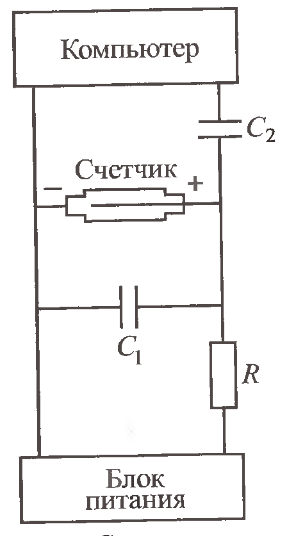
\includegraphics[width = 5cm]{inside}}
	\caption{Схема включения счетчика}
	\label{fig:image}
\end{figure}

Постоянное напряжение подается на счетчик от блока питания через сопротивление $R$. В исходном состоянии электроды и конденсатор $C_1$ заряжены до напряжения 400 В. Разделительный конденсатор $C_2$ не пропускает постоянное напряжение источника питания в интерфейсные схемы компьютера.

При возникновении тока через счетчик заряд на датчике и конденсаторе $C_1$ обеспечивает развитиеэлектронной лавины на короткое время. В процессе разряда энергия поступает от заряженного кондснснтора $C_1$, подсоединенного параллельно счетчику. Разряд в счетчике прекратится, когда напряжение на счетчике уменьшится до значения при котром разность потенциалов внутри счетчика на длине свободного пробега электрона не превышает потенциала ионизации. За время порядка нескольких $RC_1$ схема приходит в исходное состояние. При этом через конденсатор $C_2$ в электронную схему интерфейса компьютера будет передан короткий импульс.

Емкость конденсатора $C_1$ не должна быть ни слишком милой, ни слишюм большой. Запасенной в конденсаторе энергии должно хватать на создание лавинного процесса, но вместе с тем время зарядки конденсатора от блока питания ($\tau~\sim~RC_1$)‚ $~$ называемое мертвым временем счетчика, не должно быть слишком большим, так как в течение этого времени счетчик не может регистрировать частицы (обычно мертвое время составялет несколько микросекунд). В нашей установке этим условиям вполне удовлетворяет емкость самого счетчика, и конденсатор $C_1$ отсутствует.

Сопротивление резистора $R$ также не должно быть ни слишком большим (это увеличивает мертвое время штчика), ни слишком малым, чтобы конденсатор за время разряда не успевал существенно зарядиться и лавина гасла. Обычно $~$ $R~\sim~1\text{МОм}$.

Число зарегистрированных частиц зависит от времени измерения, размеров счетчика, состава газа и давления в нем, а также от материала, из которого сделаны стенки счетчика. Значительную часть регистрируемых частиц составляет естественный радиоактивный фон.

Вариации потока частиц, которые существены при измерениях в данной работе, связаны с кратковременными вариациями условий его
возникновения и распространения в атмосфере Земли. Как уже говорилось, в данной работе измеряется величина (плотность потока частиц), которая меняется со временем случайным образом. Методы обработки результатов те же, что и для рассчета случайных погрешностей.Что касается погрешности измерений потока частиц с помощтю счетчика Гейгера-Мюллера, то оценки показывают, что они малы по сравнению с изменениями самого потока или, как говорят, с флуктуациями потока. Погрешности измерений определяются в основном временем, в течение когорого восстанавливаются нормальные условия в счетчике после прохождения каждой частицы и срабатывания счетчика. Это время называтся временем разрешения. Размеры счетчика должны быть такими, чтобы время между попаданиями частиц в счетчик было больше времени разрешения.

В данной рабоче измеряется число частиц, проходящих через счетчик за 10 и 40 секунд. Выбор времен измерения связан с тем, чтобы можно было убедить в том, что при большем времени лучше выполняется нормальное распределение величин и гистограмма более симметрична, чем при малых временах, когда при обработке лучше было бы воспользоваться методами, основанными на распределении Пуассона. 

\vspace{0.5cm}
Среднеквадратичная ошибка числа отсчетов, измеренного за некоторый интервал времени, равна корню квадратному из среднего числа отсчетов за тот же интервал: $\sigma = \sqrt{n_0}$. Однако истинное среднее значение измеряемой величины неизвестно, потому в формулу для определения стандартной ошибки отдельного измерения приходится подставить не истинное среднее значение $n_0$, а измеренное значение $n$:

\begin{equation}
\sigma = \sqrt{n}
\end{equation}

Формула (1) показывает, что, как правило (с вероятностью 68\%)‚ измеренное число частиц $n$ отличается от искомого среднего не более чем
на $\sqrt{n}$. Результат измерений записывается так:

\begin{equation}
n_0 = n \pm \sqrt{n}
\end{equation}

Обратимся теперь к следующему важному вопросу. Пусть мы провели серию из $N$ измерений, в результате которых получены числа 
$n_1, n_2,..., n_N$. Эти результаты мы до сих пор использовали чтобы определить, как сильно значения, полученные в отдельных измерениях, отлчаются от истинного значения. Этот вопроса важен главным образом для выяснения того, насколько достоверен результат, полученный в отдельном измерении, однако можно использовать это для нахождения среднего значения с лучшей точностью. При $N$ измерениях среднее значение, очевидно, равно

\begin{equation}
<n> = \frac{1}{N} \sum_{i = 1}^N n_i
\end{equation}

\noindent а стандартную ошибку найти по формуле:

\begin{equation}
\sigma_{\text{отд}} = \sqrt{\frac{1}{N} \sum_{i = 1}^N (n_i - <n>)^2}
\end{equation}

В соответствии с формулой (1) стоит ожидать, что эта ошибка будет близка к $\sqrt{n_i}$, то есть 
$\sigma_{\text{отд}} \approx \sigma_i = \sqrt{n_i}$, где в качестве $n_i$ можно подставить любое из полученных $n$.Поскольку $n_i$ различны, то будем получать различные оценки, что вполне естественно. Ближе всего к значению $\sigma_{\text{отд}}$, определенному по формуле (4), лежит 
$\sqrt{<n>}$, т.е.

\begin{equation}
\sigma_{\text{отд}} \approx \sqrt{<n>}
\end{equation}

Величина $<n>$ из формулы (3), полученная путем усреднения результатов серии из $N$ опытов, не вполне совпадает с $n_0$ и сама является сучайной величиной. Теория вероятностей показывает, что стандартная ошибка отклонения $<n>$ от $n_0$ может быть определена так:

\begin{equation}
\sigma_{<n>} = \frac{1}{N} \sqrt{\sum_{i = 1}^N (n_i - <n>)^2} = \frac{\sigma_{\text{отд}}}{\sqrt{N}}
\end{equation}

\noindent При написании второй части равенства мы использовали (4).

Обычно наибольший интерес представляет на абсолютная, а относительная точность измерений. Для рассмотренной серии из $N$ измерений относительная ошибка отдельного измерения (ожидаемое отличие $<n>$ от $n_0$)

\begin{equation}
\varepsilon_{\text{отд}} = \frac{\sigma_{\text{отд}}}{n_i} \approx \frac{1}{\sqrt{n_i}}
\end{equation}

Аналогично определяется относительная ошибка в определении среднего по всем занчениям $<n>$:

\begin{equation}
\varepsilon_{<n>} = \frac{\sigma_{<n>}}{<n>} = \frac{\sigma_{\text{отд}}}{<n>\sqrt{N}} \approx \frac{1}{\sqrt{<n>N}}
\end{equation}

При написании последнего из равенств (7) значение $\sigma_{\text{отд}}$ было подставлено из формулы (5).

Таким образны, относительная точность измерения $<n>$ определяется только полным числом отсчетов и не зависит от интервалов разбиения серии (по 10, 40 или 100 с). Этого, конечно, и следовало ожидать, так как все измерения вместе составляют одно более продолжительное измерение, в котором всего зарегистрировано $\sum n_i = <n>N$ отсчетов. Как мы видим, относителъная точность измерения постепенно улучшается с увеличением числа отсчетов (а значит, и с увеличением полного времени измерений).

С помощью формулы (7) найдем, что для измерения интенсивности
космического излучения с точностью до 1\% необходимо получить, по крайней мере, $100^2 = 10000$ отсчетов, для точности 3\% достаточно 1000 отсчетов, при точноеги 10\% нужно всею 100 отсчетов и т.д. При этом точность измерения не зависит от того, получены ли все 1000 или 10 000 отсчетов в одном или нескольких независимых опытах.

\vspace{1cm}
\textbf{Приступаем к работе}

\vspace{0.5cm}
Ознакомившись с устройством установки, включим компьютер и запустим программу STAT. Для начала проведем демонстрационный эксперимент, который позволит ознакомиться с основным экспериментом. Проведя его, займемся основным. 

Подождем, пока компьютер снимет измерения. Получим таблицу данных, на основании которых мы можем построить необходимые гистограммы.

\newpage
\begin{center}
\begin{figure}[h!]
	\center{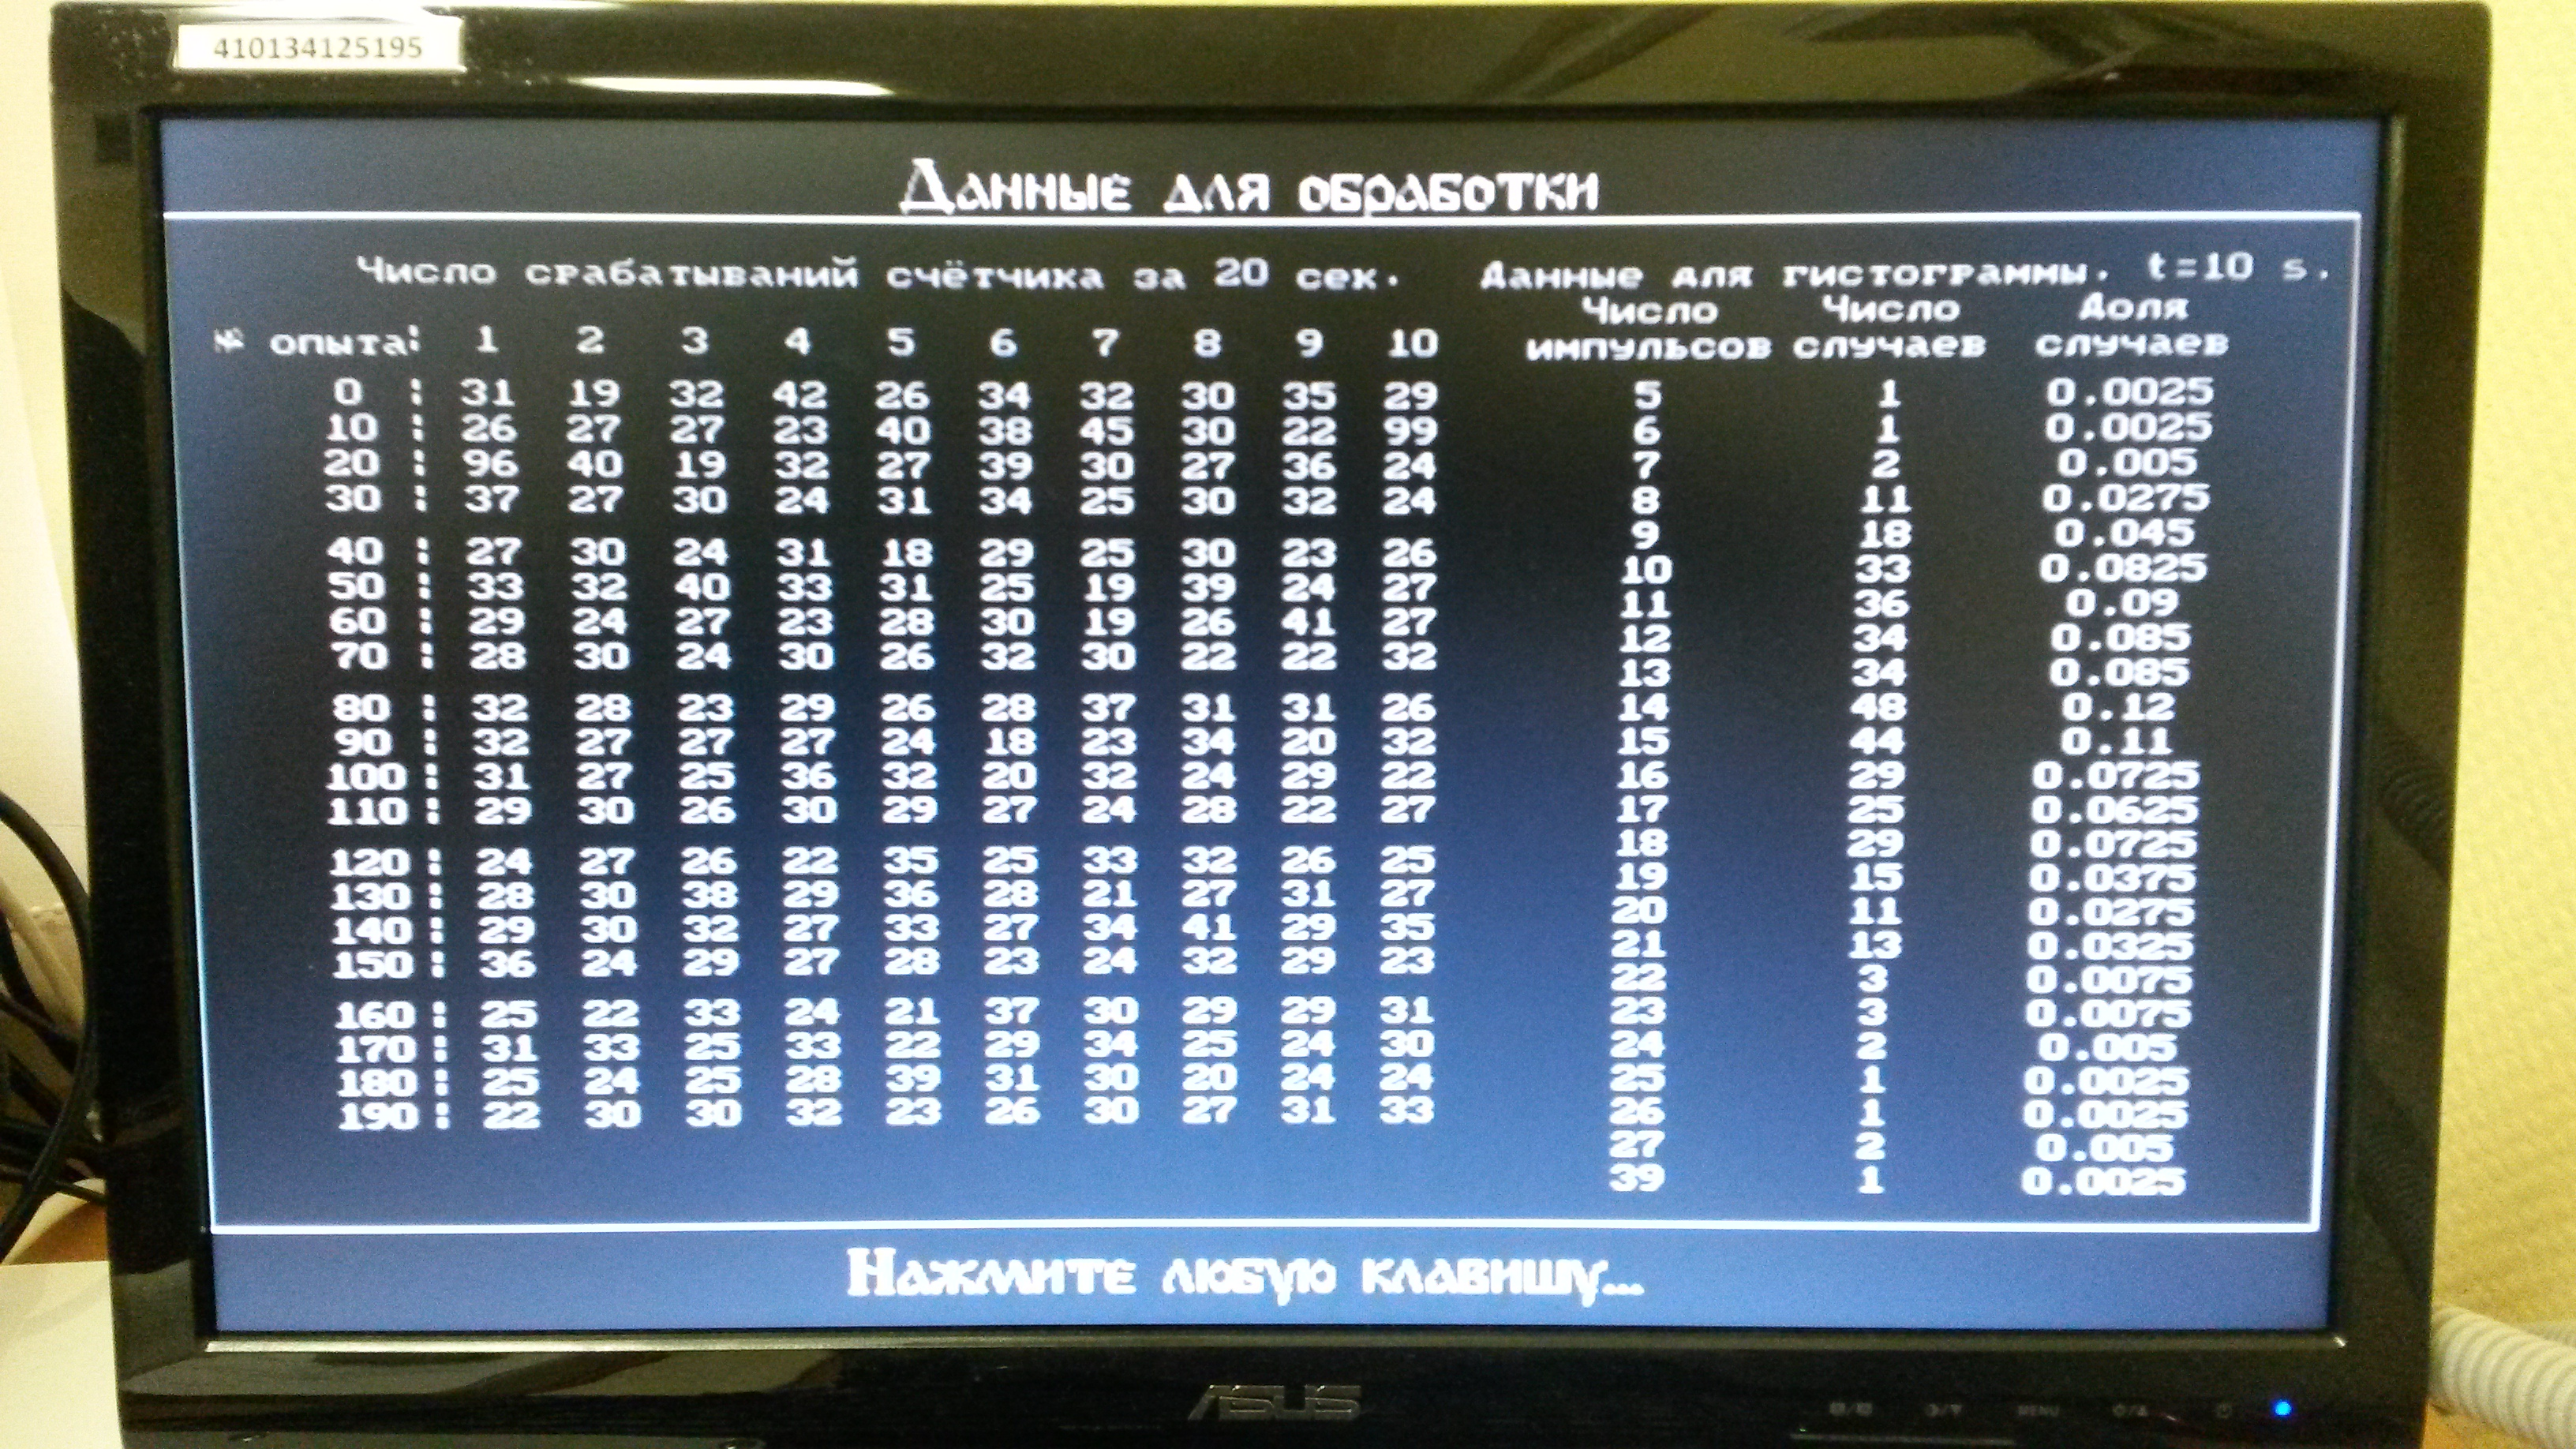
\includegraphics[width = 15cm]{table}}
	\caption{Таблица измерений}
\end{figure}
\end{center}

Отсюда можно построить гистрограмму, отражающую зависимость $\omega$ от $n$, где 

$$\omega = \frac{\text{число случаев, когда за 10 с прилетело n частиц}}{\text{полное число измерений N}}$$

\vspace{1cm}

\begin{flushleft}
\begin{tikzpicture}
\begin{axis}[
	height = 9cm,
	width  = 14cm,
	every axis y label/.style={at = {(ticklabel cs: 0.5)}, rotate = 90, anchor = near ticklabel},
	xlabel = {$n, \text{частиц/10 с}$},
	ylabel = {$\omega$}
]
\addplot+[ybar] coordinates{
	(5,  0.0025)
	(6,  0.0025)
	(7,  0.0050)
	(8,  0.0275)
	(9,  0.0450)
	(10, 0.0825)
	(11, 0.0900)
	(12, 0.0850)
	(13, 0.0850)
	(14, 0.1200)
	(15, 0.1100)
	(16, 0.0725)
	(17, 0.0625)
	(18, 0.0725)
	(19, 0.0375)
	(20, 0.0275)
	(21, 0.0325)
	(22, 0.0075)
	(23, 0.0075)
	(24, 0.0050)
	(25, 0.0025)
	(26, 0.0025)
	(27, 0.0050)
	(39, 0.0025)
};
\end{axis}
\end{tikzpicture}
\end{flushleft}











\end{document}